%
%  test-1.tex
%  artificial intelligence
%
%  Created by Illya Starikov on Saturday, July 15, 2018.
%  Copyright 2018. Illya Starikov. All rights reserved.
%

\RequirePackage[l2tabu, orthodox]{nag}
\documentclass[12pt]{scrartcl}

\newcommand{\exercisenumber}{2}
\newcommand{\duedate}{July 29\textsuperscript{th}, 2018}
\usepackage{amssymb,amsmath,verbatim,graphicx,microtype,upquote,units,booktabs,akkwidepage}

\newcommand{\chapterNumber}[1]{
    \setcounter{section}{#1}
    \addtocounter{section}{-1}
}
\usepackage{multicol}
\usepackage[shortlabels]{enumerate}

\title{Test \#2}

\begin{document}
\maketitle

\section{C4.5}
\begin{center}
    \textit{Split = 120}
    \begin{align*}
        \text{EntropyLT} &= % 3 False, 1 True
            -\nicefrac{3}{4}\,\log_2\left(\nicefrac{3}{4}\right)
            -\nicefrac{1}{4}\,\log_2\left(\nicefrac{1}{4}\right) \\
        \text{EntropyGt} &= % 2 False, 3 True
            -\nicefrac{2}{5}\,\log_2\left(\nicefrac{2}{5}\right)
            -\nicefrac{3}{5}\,\log_2\left(\nicefrac{3}{5}\right) \\
        \text{Info Gain} &=
            X - \left(\nicefrac{4}{9} \times \text{EntropyLT} + \nicefrac{5}{9} \times \text{EntropyGT}\right)
    \end{align*}

    \textit{Split = 140}
    \begin{align*}
        \text{EntropyLT} &= % 4 False, 2 True
            -\nicefrac{4}{6}\,\log_2\left(\nicefrac{4}{6}\right)
            -\nicefrac{2}{6}\,\log_2\left(\nicefrac{2}{6}\right) \\
        \text{EntropyGt} &= % 2 False, 1 True
            -\nicefrac{2}{3}\,\log_2\left(\nicefrac{2}{3}\right)
            -\nicefrac{1}{3}\,\log_2\left(\nicefrac{1}{3}\right) \\
        \text{Info Gain} &=
            X - \left(\nicefrac{6}{9} \times \text{EntropyLT} + \nicefrac{3}{9} \times \text{EntropyGT}\right)
    \end{align*}

    We choose the split that we calculated previously based on it's associated \textbf{highest information gain}. Values before it should be assigned \textit{Less Than Split} and values after it should be assigned \textit{Greater Than Split}.
\end{center}


\section{Grouping Or Splitting}
\begin{center}
    \textit{\{\{SciFiction, Mystery\}, \{NonFiction\}\}}
    \begin{align*}
        \text{SciMystery} &= % 3 Rock, 2 Country, 1 Classical
            -\nicefrac{3}{6}\,\log_2\left(\nicefrac{3}{6}\right)
            -\nicefrac{2}{6}\,\log_2\left(\nicefrac{2}{6}\right)
            -\nicefrac{1}{6}\,\log_2\left(\nicefrac{1}{6}\right) \\
        \text{NonFiction} &= % 0 Rock, 1 Country, 1 Classical
            - 0
            -\nicefrac{1}{6}\,\log_2\left(\nicefrac{1}{6}\right)
            -\nicefrac{1}{6}\,\log_2\left(\nicefrac{1}{6}\right) \\
        \text{Info Gain} &=
            1.5575 - \left(\nicefrac{6}{8} \times \text{SciMystery} + \nicefrac{2}{8} \times \text{NonFiction}\right)
    \end{align*}

    \textit{\{\{SciFiction, NonFiction\}, \{Mystery\}\}}
    \begin{align*}
        \text{SciNonFiction} &= % 2 Rock, 1 Country, 1 Classical
            -\nicefrac{2}{4}\,\log_2\left(\nicefrac{2}{4}\right)
            -\nicefrac{1}{4}\,\log_2\left(\nicefrac{1}{4}\right)
            -\nicefrac{1}{4}\,\log_2\left(\nicefrac{1}{4}\right) \\
        \text{NonFiction} &= % 1 Rock, 2 Country, 1 Classical
            -\nicefrac{1}{4}\,\log_2\left(\nicefrac{1}{4}\right)
            -\nicefrac{2}{4}\,\log_2\left(\nicefrac{2}{4}\right)
            -\nicefrac{1}{4}\,\log_2\left(\nicefrac{1}{4}\right) \\
        \text{Info Gain} &=
            1.5575 - \left(\nicefrac{4}{8} \times \text{SciNonFiction} + \nicefrac{4}{8} \times \text{Mystery}\right)
    \end{align*}

    \textit{\{\{Mystery, NonFiction\}, \{NonFiction\}\}}
    \begin{align*}
        \text{SciNonFiction} &= % 1 Rock, 3 Country, 2 Classical
            -\nicefrac{1}{6}\,\log_2\left(\nicefrac{1}{6}\right)
            -\nicefrac{3}{6}\,\log_2\left(\nicefrac{3}{6}\right)
            -\nicefrac{2}{6}\,\log_2\left(\nicefrac{2}{6}\right) \\
        \text{NonFiction} &= % 2 Rock, 0 Country, 0 Classical
            -\nicefrac{2}{2}\,\log_2\left(\nicefrac{2}{2}\right)
            - 0
            - 0 \\
        \text{Info Gain} &=
            1.5575 - \left(\nicefrac{6}{8} \times \text{SciNonFiction} + \nicefrac{2}{8} \times \text{NonFiction}\right)
    \end{align*}

    To determine if any attributes are to be grouped, take the \textbf{highest information gain}, and compare it to the Entropy Before Split for music preference. If information gain is higher, then the grouping was better; if not, the grouping was worse.
\end{center}


\section{Support Vectors}
The equations would reduce down to:

\begin{align*}
    10\, \alpha_1 + 10\, \alpha_2 &= -1 \\
    10\, \alpha_1 + 11\, \alpha_2 &= 1 \\
\end{align*}

For which we get the following solutions:

\begin{equation*}
    \alpha_1 = -\frac{21}{10} \qquad \alpha_2 = 2
\end{equation*}

For the discriminating 2D hyperplane, we get as follows:

\begin{align*}
    w &= -\frac{21}{10}\times s_1 + 2\times s_2 \\
      &= <-\frac{3}{10}, 2, -\frac{41}{10}>
\end{align*}

Meaning our equation would be as follows:

\begin{equation*}
    -\nicefrac{3}{10}\, x - 2\, y -\nicefrac{41}{10} = 0
\end{equation*}

\section{Bayesian Network}
The algorithm will enumerate the possible options (in the original ordering) for a parent of X2. It does so by calculating the probability of the particular attribute being a parent of X2, and the one with the greatest probability is the node that becomes the parents.

\begin{enumerate}
    \item  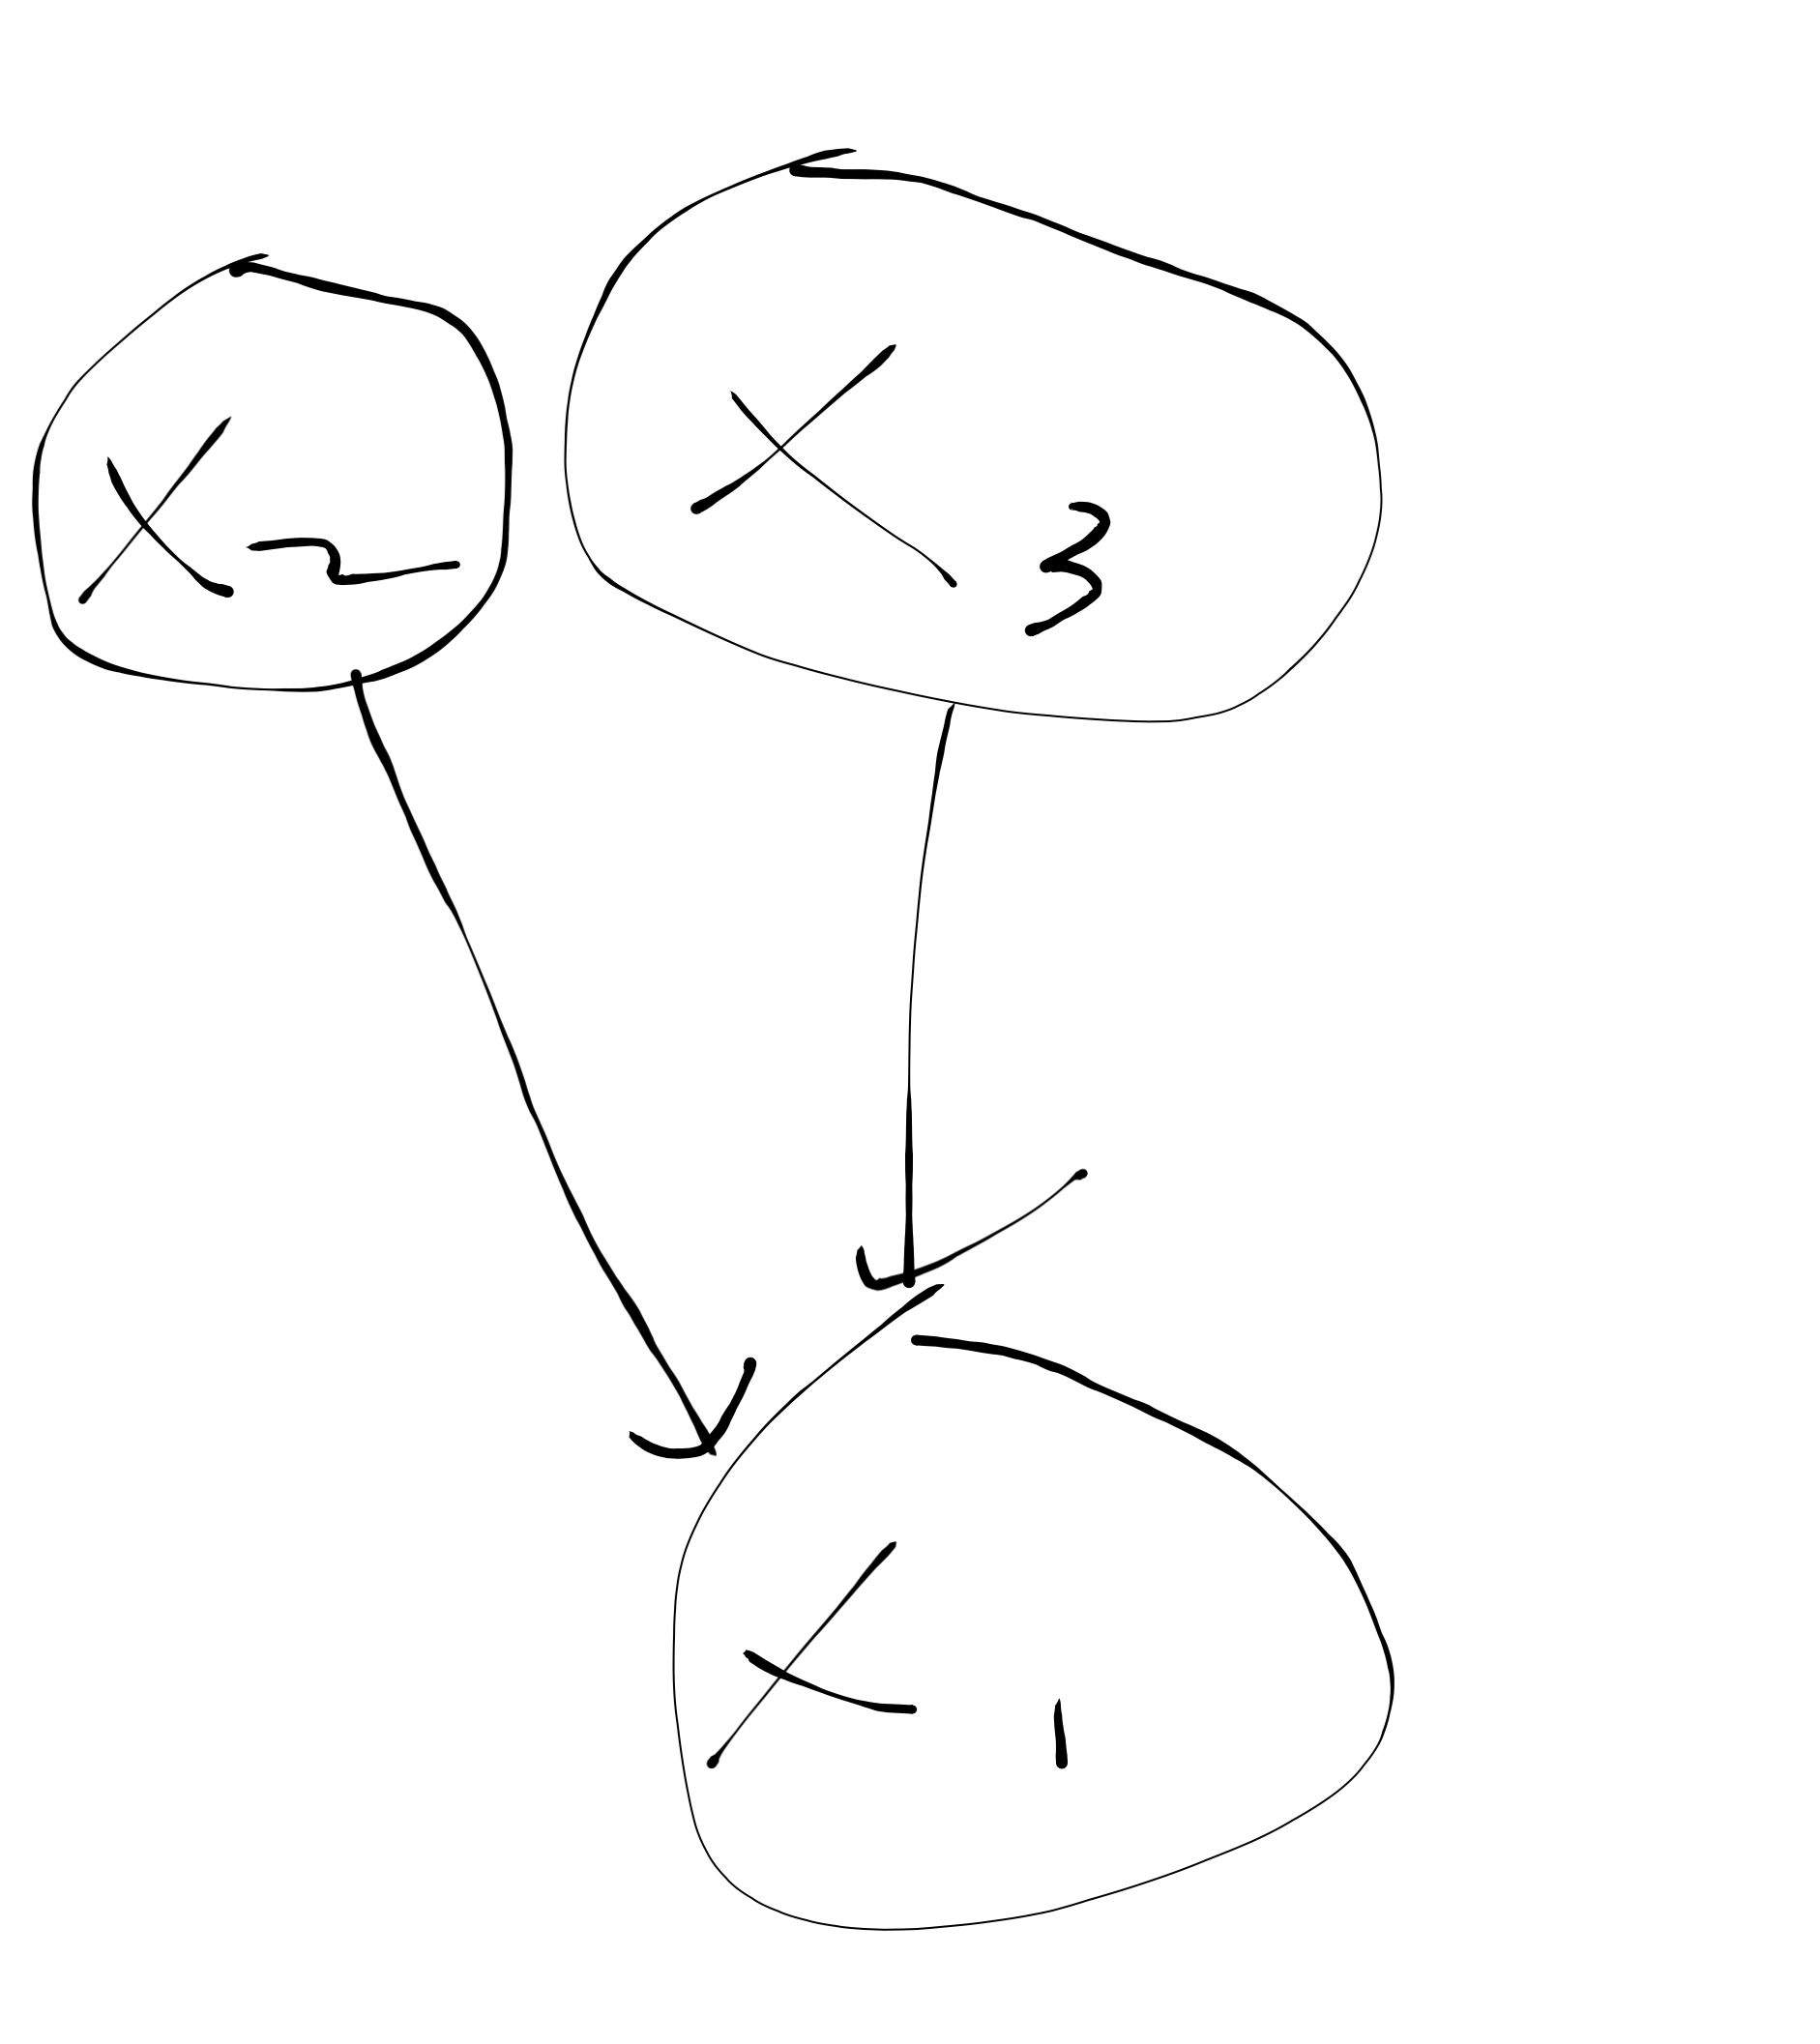
\includegraphics[width=.5\textwidth]{assets/1}
    \item  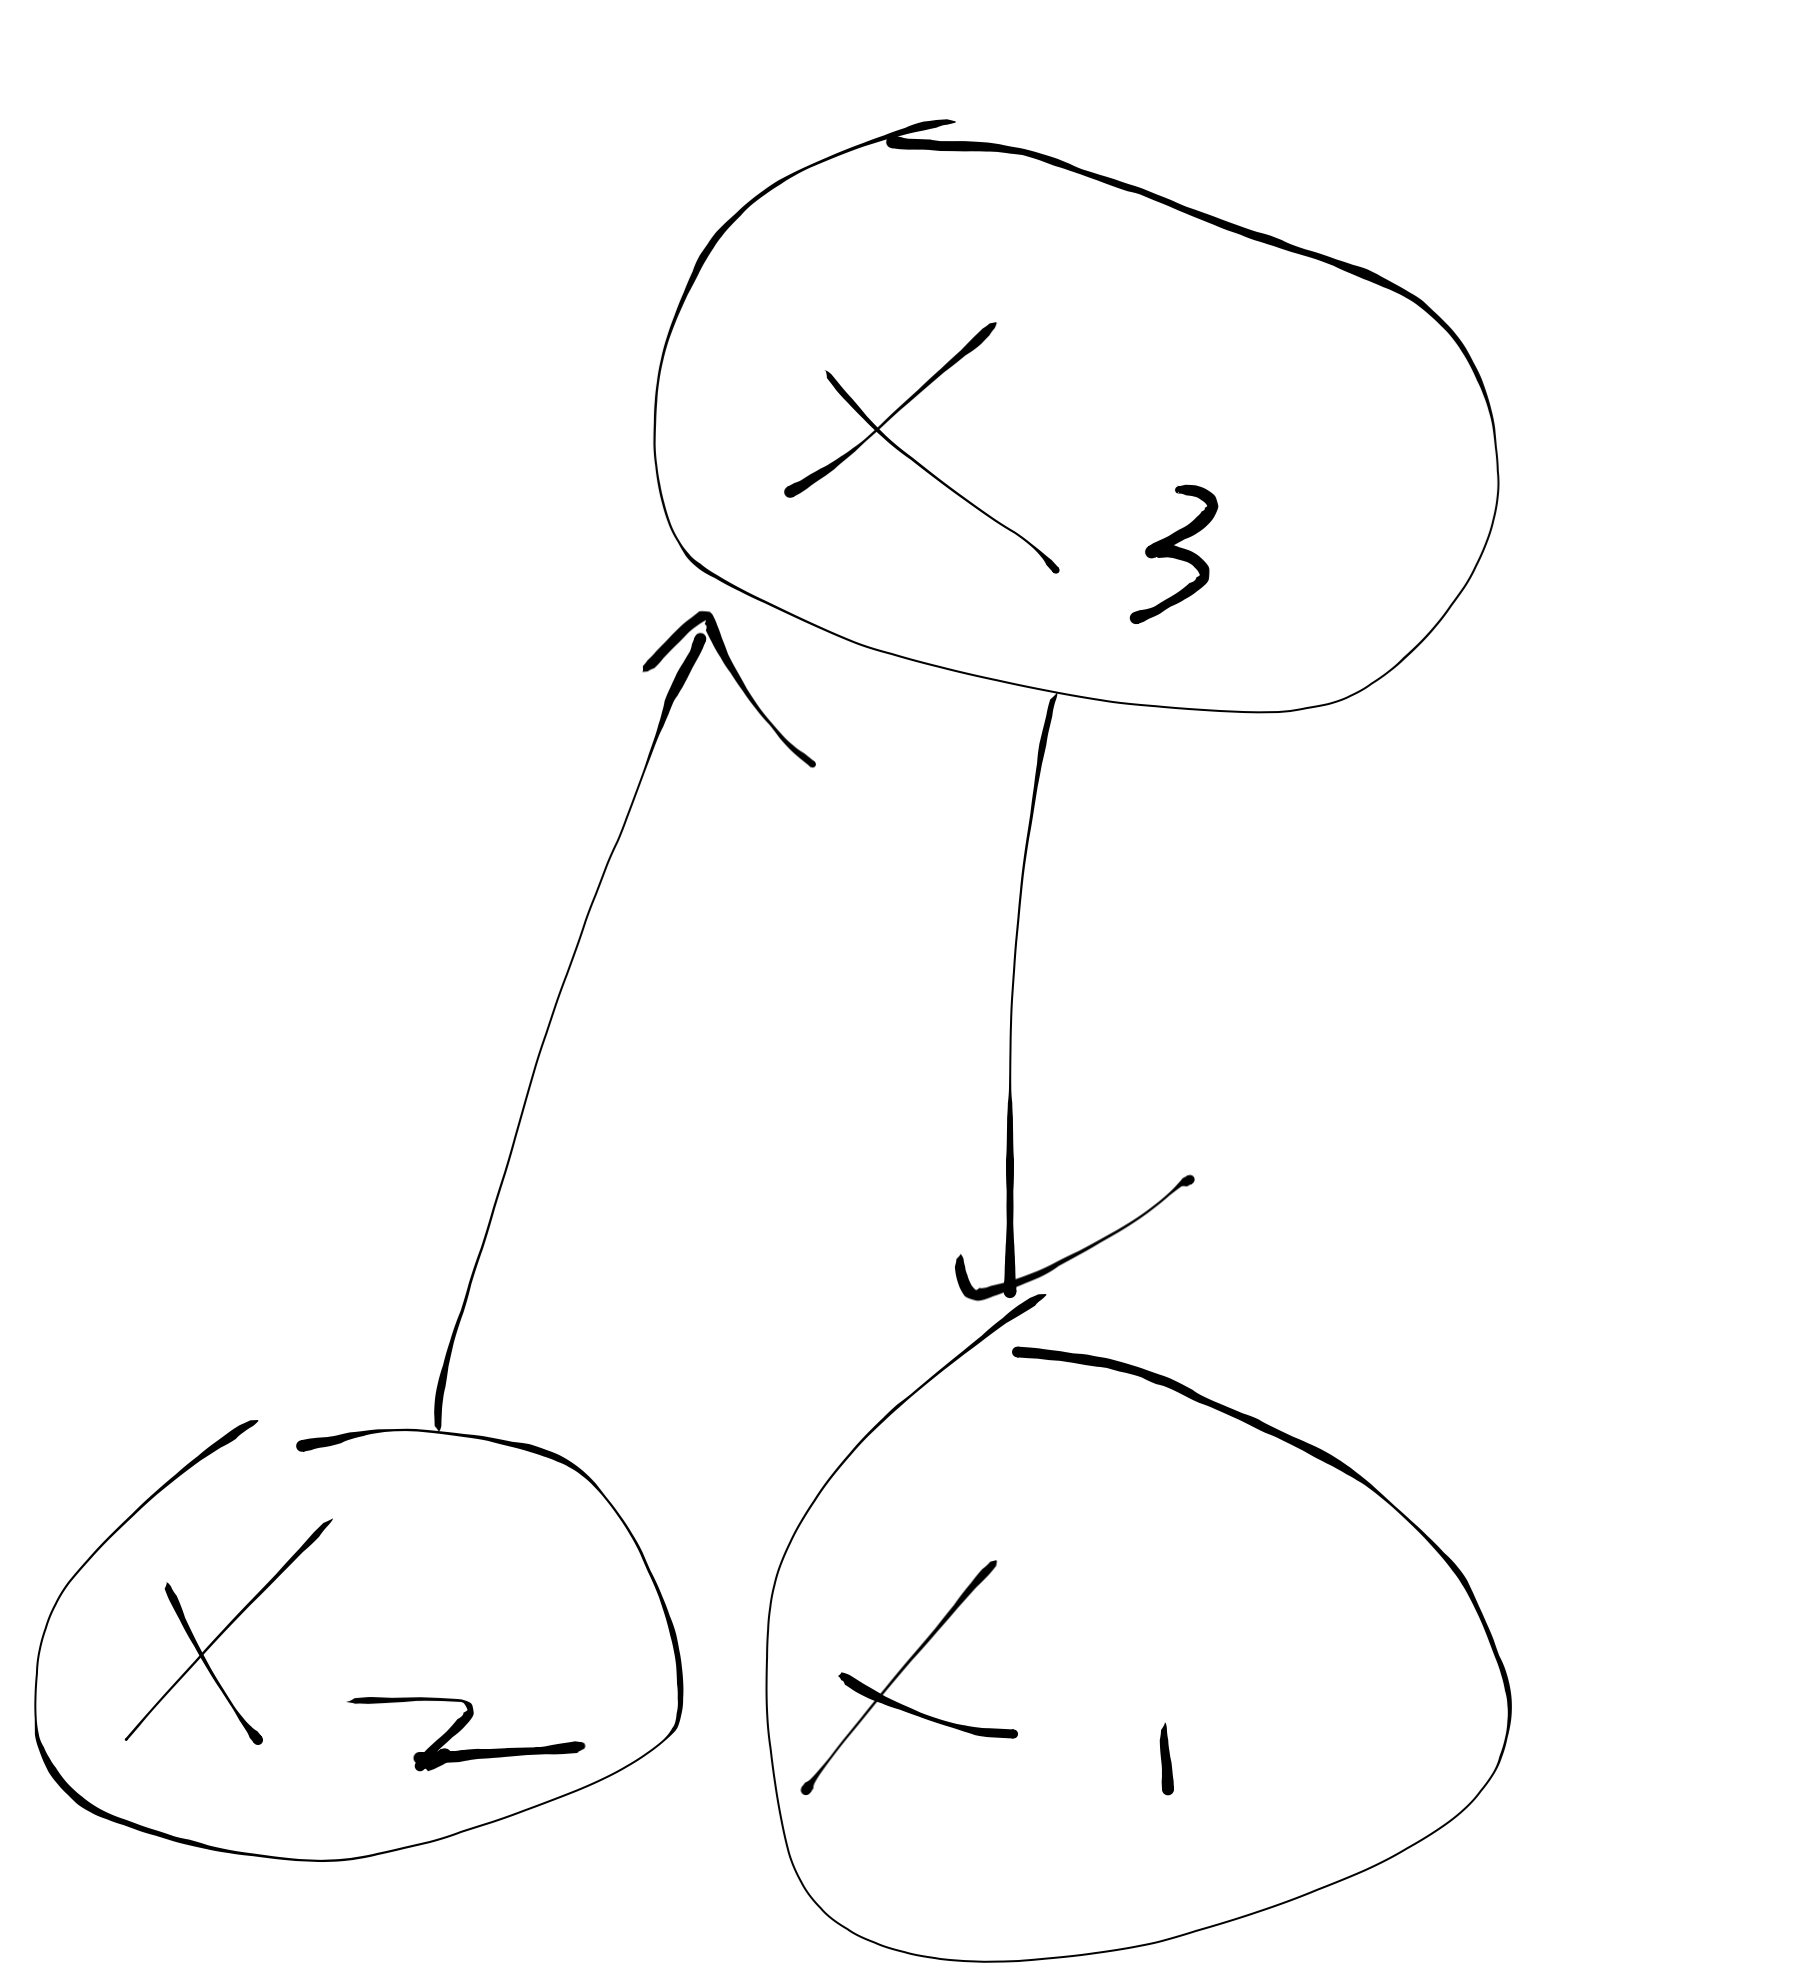
\includegraphics[width=.5\textwidth]{assets/2}
    \item  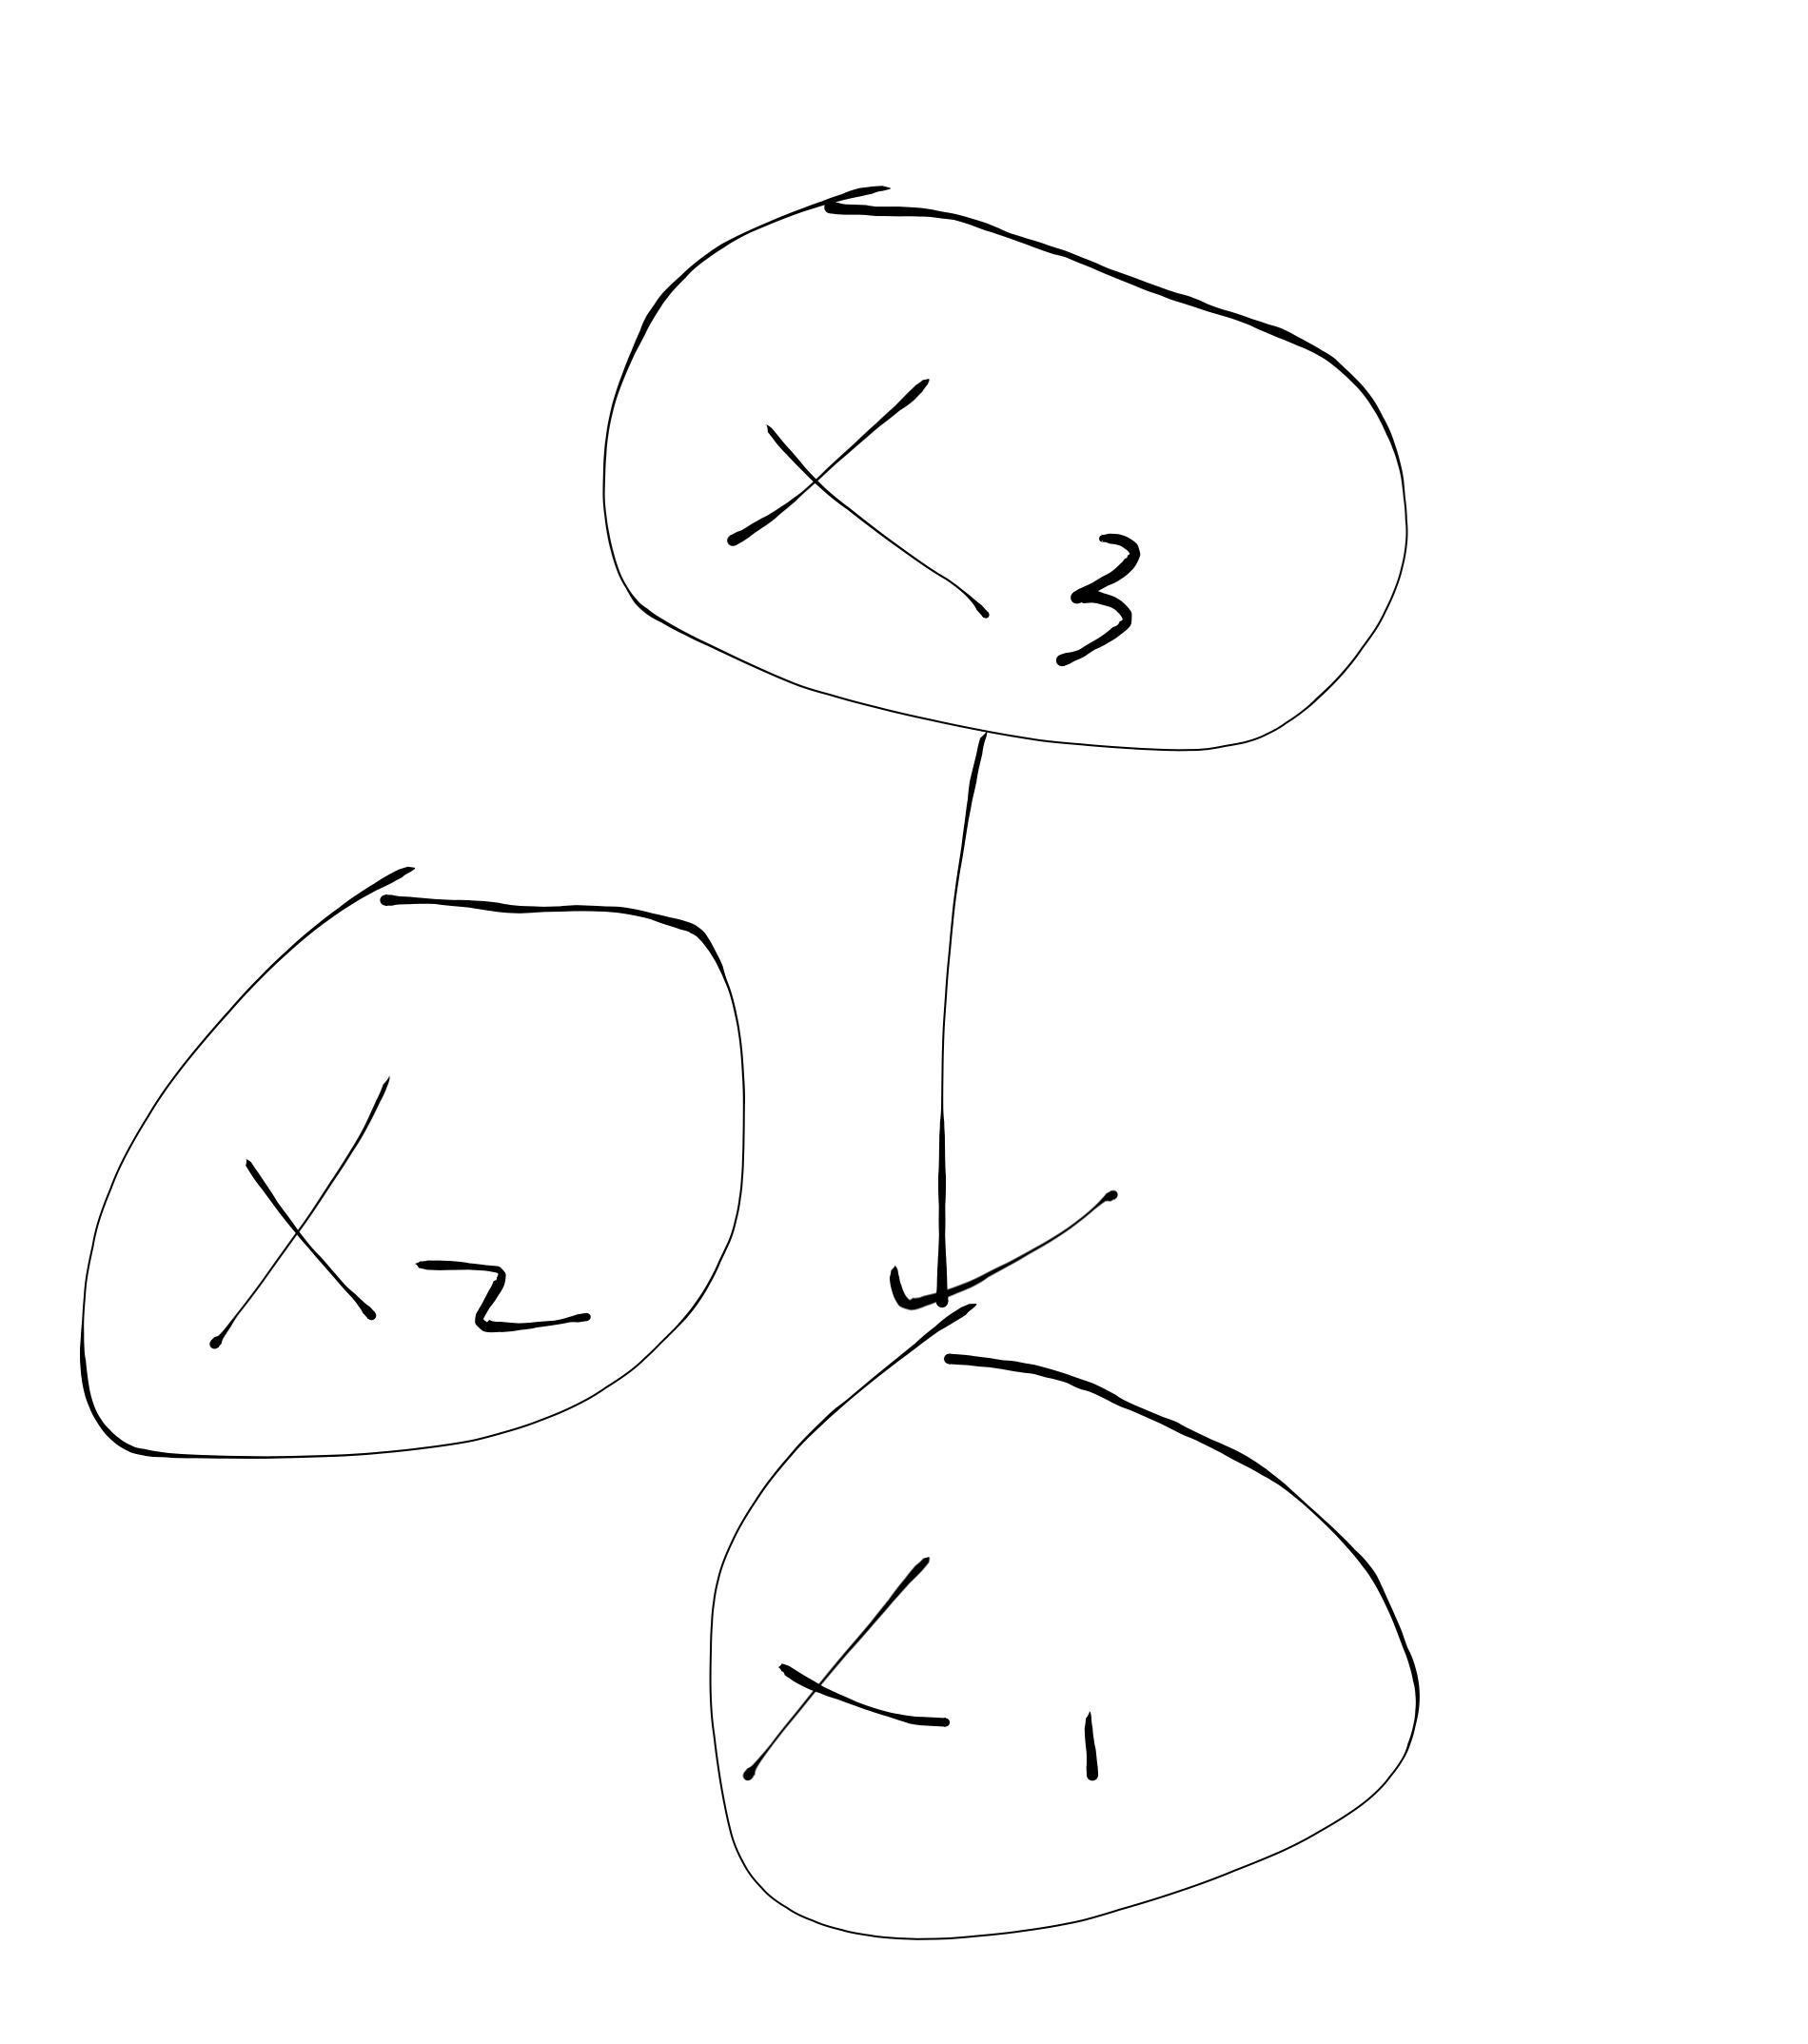
\includegraphics[width=.5\textwidth]{assets/3}
\end{enumerate}

\section{DBScan}
\begin{table}[H]
    \centering
    \begin{tabular}{|c|c|l|}
        \hline
            & density & designation \\\hline
        A1  & 2 & Border \\
        A2  & 2 & Border \\
        A3  & 3 & Core \\
        A4  & 1 & Noise \\
        A5  & 2 & Border \\
        A6  & 2 & Border \\
        A7  & 2 & Noise \\
        A8  & 1 & Noise \\
        A9  & 2 & Noise \\
        A10 & 3 & Core \\\hline
    \end{tabular}
\end{table}

The clusters would be as follows: $\{A1, A2, A3\}$ and $\{A5, A6, A10\}$. Points with have are dense (density > number of points) are designated as core points. Points that are around a core points (within an $\epsilon$ of a core point) are designated as border point. Points that fall in neither of these categories are designated as noise.

\section{Linkage}
The single linkage would be as follows:

\begin{equation*}
    \left| (1,\, 4) - (3,\,5) \right| = 3
\end{equation*}

The complete linkage would be as follows:

\begin{equation*}
    \left| (1,\, 2) - (4,\,5) \right| = 6
\end{equation*}

The centroid linkage would be as follows:

\begin{equation*}
    \left| (1,\, \nicefrac{11}{4}) - (\nicefrac{14}{4},\, 5) \right| = \nicefrac{19}{4}
\end{equation*}

The average linkage would be as follows:

\begin{equation*}
    \text{Average of all distances between points} = 5
\end{equation*}

\section{Ensemble Classifier}

\begin{table}[H]
    \centering
    \begin{tabular}{|l|c|c|c|c|}
        \hline
        Sum & -2 & 4 & -6 & 2 \\\hline
        Class & -1 & 1 & -1 & 1 \\
        \hline
    \end{tabular}
\end{table}

\section{Bayes Network}
For \textbf{worker = T}, the likelihood would be as follows:

\begin{equation*}
    0.8 \times 0.02 \times 0.1 \times 0.1 \times 0.01
\end{equation*}

For \textbf{worker = F}, the likelihood would be as follows:

\begin{equation*}
    0.8 \times 0.02 \times 0.1 \times 0.1 \times 0.99
\end{equation*}

The probability for \textbf{worker = T} would be:

\begin{equation*}
    \frac{0.8 \times 0.02 \times 0.1 \times 0.1 \times 0.01}{0.8 \times 0.02 \times 0.1 \times 0.1 \times 0.01 + 0.8 \times 0.02 \times 0.1 \times 0.1 \times 0.99}
\end{equation*}

And the probability for \textbf{worker = F} would be:

\begin{equation*}
    \frac{0.8 \times 0.02 \times 0.1 \times 0.1 \times 0.99}{0.8 \times 0.02 \times 0.1 \times 0.1 \times 0.01 + 0.8 \times 0.02 \times 0.1 \times 0.1 \times 0.99}
\end{equation*}


\section*{Multiple Choice}
\begin{enumerate}
    \setcounter{enumi}{8}

    \item d. repeatedly sampling from the original dataset according to a uniform probability distribution
    \item c. increased, decreased
    \item a. bias, variance
    \item b. false
    \item c. 180 instances reached this point in the decision tree, but 22 of those were not classified as tested\_negative in the training dataset
    \item d. age > 34
    \item b. compute the predicted error rate of the rule with one condition (C1, C2, C3) deleted and no conditions deleted, and, from those, use the version of the rule with the lowest rate
    \item c. each instance in the dataset will have a probability of being in a particular cluster
    \item b. supervised


\end{enumerate}


\end{document}
